\documentclass{sigchi}

% Use this section to set the ACM copyright statement (e.g. for
% preprints).  Consult the conference website for the camera-ready
% copyright statement.

% Copyright
\CopyrightYear{2016}
%\setcopyright{acmcopyright}
\setcopyright{acmlicensed}
%\setcopyright{rightsretained}
%\setcopyright{usgov}
%\setcopyright{usgovmixed}
%\setcopyright{cagov}
%\setcopyright{cagovmixed}
% DOI
\doi{http://dx.doi.org/10.475/123_4}
% ISBN
\isbn{123-4567-24-567/08/06}
%Conference
\conferenceinfo{CHI'16,}{May 07--12, 2016, San Jose, CA, USA}
%Price
\acmPrice{\$15.00}


% Load basic packages
\usepackage{balance}       % to better equalize the last page
\usepackage{graphics}      % for EPS, load graphicx instead 
\usepackage[T1]{fontenc}   % for umlauts and other diaeresis
\usepackage{txfonts}
\usepackage{mathptmx}
\usepackage[pdflang={en-US},pdftex]{hyperref}
\usepackage{color}
\usepackage{booktabs}
\usepackage{textcomp}

% Some optional stuff you might like/need.
\usepackage{microtype}        % Improved Tracking and Kerning
% \usepackage[all]{hypcap}    % Fixes bug in hyperref caption linking
\usepackage{ccicons}          % Cite your images correctly!
% \usepackage[utf8]{inputenc} % for a UTF8 editor only

% If you want to use todo notes, marginpars etc. during creation of
% your draft document, you have to enable the "chi_draft" option for
% the document class. To do this, change the very first line to:
% "\documentclass[chi_draft]{sigchi}". You can then place todo notes
% by using the "\todo{...}"  command. Make sure to disable the draft
% option again before submitting your final document.
\usepackage{todonotes}

% Paper metadata (use plain text, for PDF inclusion and later
% re-using, if desired).  Use \emtpyauthor when submitting for review
% so you remain anonymous.
\def\plaintitle{ForceScroll and ForcePress: Enhance Reading Speed Using Force Touch Technique}
\def\plainauthor{First Author, Second Author, Third Author,
  Fourth Author, Fifth Author, Sixth Author}
\def\emptyauthor{}
\def\plainkeywords{Human Computer Interaction; Trackpad; Force Touch; Experiment.}
\def\plaingeneralterms{Documentation, Standardization}

% llt: Define a global style for URLs, rather that the default one
\makeatletter
\def\url@leostyle{%
  \@ifundefined{selectfont}{
    \def\UrlFont{\sf}
  }{
    \def\UrlFont{\small\bf\ttfamily}
  }}
\makeatother
\urlstyle{leo}

% To make various LaTeX processors do the right thing with page size.
\def\pprw{8.5in}
\def\pprh{11in}
\special{papersize=\pprw,\pprh}
\setlength{\paperwidth}{\pprw}
\setlength{\paperheight}{\pprh}
\setlength{\pdfpagewidth}{\pprw}
\setlength{\pdfpageheight}{\pprh}

% Make sure hyperref comes last of your loaded packages, to give it a
% fighting chance of not being over-written, since its job is to
% redefine many LaTeX commands.
\definecolor{linkColor}{RGB}{6,125,233}
\hypersetup{%
  pdftitle={\plaintitle},
% Use \plainauthor for final version.
%  pdfauthor={\plainauthor},
  pdfauthor={\emptyauthor},
  pdfkeywords={\plainkeywords},
  pdfdisplaydoctitle=true, % For Accessibility
  bookmarksnumbered,
  pdfstartview={FitH},
  colorlinks,
  citecolor=black,
  filecolor=black,
  linkcolor=black,
  urlcolor=linkColor,
  breaklinks=true,
  hypertexnames=false
}

% create a shortcut to typeset table headings
% \newcommand\tabhead[1]{\small\textbf{#1}}

% End of preamble. Here it comes the document.
\begin{document}

\title{\plaintitle}

\numberofauthors{2}
\author{%
  \alignauthor{Ruoteng Ma\\
    \affaddr{University of Waterloo}\\
    \affaddr{Waterloo, Canada}\\
    \email{ruoteng.ma@uwaterloo.ca}}\\
  \alignauthor{Sung-Shine Lee\\
    \affaddr{University of Waterloo}\\
    \affaddr{Waterloo, Canada}\\
    \email{s469lee@uwaterloo.ca}}
}




\maketitle

\begin{abstract}
  With the increasing availability of digital literatures, reading using digital devices have became common practice. While mobile devices removed the need of carrying physical books, navigating through a digital document can also be a challenging task. Without the help of mouse and physical keyboard, digital devices usually rely on trackpad interactions to enable navigation. In recent years, a number of devices have started to take the amount of forces applied during the trackpad interaction into consideration. In this paper, we present ForceScroll and ForcePress, two novel interaction techniques that utilize the new interaction dimensions added by force touch to improve the interaction experience provided by the traditional trackpad control scheme. Both systems were implemented using JavaScript. We present a series of experiments comparing the ForceScroll and ForcePress against traditional trackpad control technique, in which we examine the error rate and efficiency of the new systems. The main contribution of paper is that we proposed two new interaction techniques and conducted user study to check their performance against the existing technique.  
\end{abstract}

\category{H.5.2.}{Information Interfaces and Presentation
  (e.g. HCI)}{User Interfaces
  - Input devices and strategies} \category{}{}{}

\keywords{\plainkeywords}

\section{Introduction}

Book readers use their fingers to turn the pages of the book they are reading, they can easily control the amount of pages they are turning and quickly reach desired location. A larger amount of existing literatures are presented as digital documents, readable on devices such as Personal Computers and Laptops. For reading digital documents on these devices, the task of efficiently moving between pages and find desired contents can be difficult to achieve. Personal computers and laptops allow users to control their devices using physical keyboard and mouse, this gives user a reliable and easy way to navigate the document. However, problem arises for laptop users without access to mouse, who perform their interaction using trackpad. Without the support of physical mouse, viewing documents on these devices can be inefficient. 

%Different types of digital documents also provide different ways of traversal. Documents with well defined pages could be traversed by going directly to a specified page; documents that have a table-of-contents which is linked to well-defined sections allow users to go directly to desired chapter or section of the document, regardless of the length of the document; documents without any of the above functions will need to be traversed by moving through the entire document sequentially. 


ForceScroll and ForcePress present two alternative control schemes for devices that support force-sensitive trackpad. We want to design new viewing control schemes for these devices by applying force touch. We believe that with the help of force touch, the efficiency of trackpad control can be improved. 


Digital documents can also have different designs and functionalities. For ForceScroll and ForcePress, we assume all documents viewed on the device have well-defined and linked pages and sections, which allows users to jump to certain location within the document. For the purpose of evaluation the new technique, we are only interested in the improvement ForceScroll and ForcePress systems have on the traditional scrolling action performed on trackpads. To test the ForceScroll and ForcePress systems in a controlled environment, we do not consider other page turning methods, such as entering a page number or using the table-of-content. We implemented both prototype systems on a MacBook Pro laptop with force-sensitive trackpad.    
  

Force touch has been explored by a number of works, Presstures \cite{rendl2014presstures} allows users to apply force to select interaction mode in order to avoid uncomfortable interactions such as pressing hard for a long distance. Heo and Lee \cite{heo2011force} designed a web browser and an e-book reader that both use force input as the main control technique and give users visual feedback on the applied force. ForceEdge \cite{antoine2017forceedge} expends the autoscroll function on touch devices with force-sensing ability, resulting in a more accurate target-seeking experience. Surale et al. \cite{surale2017experimental} explored mode-switching task with six gestures both with and without force, Taher et al. \cite{taher2014empirical} studied the characterization of input force on mobile devices and provided a baseline for further studies. Finally, Mandalapu and Subramanian \cite{mandalapu2011exploring} explored the idea of using force as an alternative to multi touch interactions. ForceScroll and ForcePress benefit from previous studies, but in the context of document viewing, there is a lack of comparison between force-enabled techniques and traditional techniques, and our ForceScroll interaction system is different from those proposed before.          


We built the ForceScroll and ForcePress application using JavaScript, the application achieved the above functionality and allowed us to test our hypotheses in a controlled environment. We evaluated the system by the time required for a user to reach a target location, the total amount of interactions, and the total overshoot distances. See Figure 1 for an illustration of the application.  




\begin{figure}[!h]
	\centering
	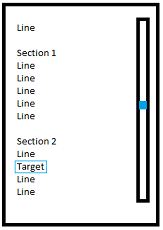
\includegraphics[width=0.9\columnwidth]{figures/Capture}
	\caption{The participants were required to move the screen until the highlighted target was on screen and click it. The location of the target and the chapter headers are displaced on the sidebar}~\label{fig:figure1}
\end{figure}


The main contribution of the paper is that we proposed novel interaction techniques that utilized the power of force touch to facilitate the page scrolling task for trackpad devices, we also performed a comparison study between the new techniques and the traditional technique where force sensing is disabled.


\section{Related Work}

\subsection{Scrolling}
As one of the most commonly used features on digital devices, scrolling as an operation has been thoroughly studied. Andersen \cite{andersen2005simple} developed a linear model for the scrolling movement time with an optical mouse and distance to target, and concluded that the scrolling movement time does not follow Fitts' law. Quinn et al. \cite{quinn2012exposing} acknowledged the difficulty in studying scrolling operation since the existing transfer functions, which can be used to alter scrolling performance, are unknown to researchers. They created a framework of transfer function factors and proposed a method to study proprietary transfer functions for different input devices. Cockburn et al. \cite{cockburn2012improving} presented three gain functions, called document-length-dependent gain, which utilize document length as an input of the function, to improve scrolling performance. Aceituno et al. \cite{aceituno2017design} studied the performance of different edge-scrolling techniques and presented a framework of factors that affect performance and design.  

A variety of alternative scrolling methods have been proposed and studied. For example, Smith and Schraefel \cite{smith2004radial} presented the radial scroll interface, which allows users to scroll up and down by performing clock and counter-clockwise gestures on a touch interface. Other than simple alternative interaction gestures, some works aimed to extend the interaction space. Takashima et al. \cite{takashima2015exploring} proposed an improved scrolling control by extending the motor space of the action. Their interface can be applied on touch devices, using either off-window touch space or mid-air motions detectable by 3D motion sensors. Push-Edge \cite{malacria2015push} detected cursor at the edge of the viewport, it captured device signals from action space outside the viewport and used them as input to a scrolling transfer function, thus altered the traditional edge-scrolling feature and kept the cursor stationary on the screen while scrolling. Other studies attempted to expend the dimension of the interaction. Miyaki and Rekimoto \cite{miyaki2009graspzoom} proposed a pressure sensing interaction technique, GraspZoom, for the scrolling task on mobile devices with an attached Force Sensitive Resistor on the back of the device. The utilization of pressure increased the dimension of interaction and allowed gestures to be augmented by pressure.  

Research has also been done on scrolling task with a focus on the trackpad. Bial et al. \cite{bial2010study} proposed a two-handed input scheme, where the trackpad was used as a dedicated scrolling device. The system also implemented different scrolling actions such as relative scrolling and flicking. Arthur et al. \cite{arthur2008evaluating} also presented a circular touch gesture called ChiralMotion that can be performed on the trackpad. The system reduces 2D motions to 1D scrolling actions.


\subsection{Force Touch}
In this section, we discuss previous works on force sensitive touch input. Taher et al. \cite{taher2014empirical} derived a ground-truth characterization of force touch gestures by performing a controlled user study; this gives a good starting point for designing input scheme using the force-sensitive technique. 


The applications of force on traditional interaction methods have been proposed and studied by many authors. Goguey et al. \cite{goguey2018improving} designed a force-sensitive text selection system that allowed different actions for each level of pressure applied. By applying different levels of force before releasing their finger, the system lets users select different portions of text centered around the touched position. Zoofing \cite{quinn2009zoofing} presented a pressure-based zooming technique as a part of their list selection interface where the level of zooming was controlled by the level of pressure applied at the zoom point. Also focused on zooming, Mandalapu and Subramanian \cite{mandalapu2011exploring} explored the possibility of using pressure as an alternative to multi-touch control. ForceEdge \cite{antoine2017forceedge} explored the use of force for trackpad autoscrolling, allowing users to control the scrolling rate by varying applied force. These works are related to ForcePress. Heo and Lee \cite{heo2011force} presented a system that augmented traditional touchscreen gestures with two levels of force, where the same gesture invoked different actions when the amount of force applied was different. They also designed two sample applications for their system. Their work is closely related to ForceScroll. 

Many research studied the effect of visualized feedback since the force touch systems could support different functionalities for different levels of force applied. Sheik-Nainar et al. \cite{sheik2013two} developed an interaction model for their TouchPad prototype that supported two levels of force, and tested how feedback can affect the performance of the system. Their user study concluded that the users prefer to have no feedback on the level of force applied, even though the feedback provided in the experiment helped them to locate the force thresholds. This could be the result of only having two levels of force present. Goguey et al. \cite{goguey2018improving} visualized the amount of pressure applied using a circular gauge that acknowledged the users their current amount of applied pressure and the level of actions it was in. Their user study discovered that the pressure gauge visualization feedback was necessary for learning the techniques. Zoofing \cite{quinn2009zoofing} provided visual feedback by displaying a red circle centered at the touch point and the level of force applied was represented by the diameter of the circle, harder the press, larger the circle. Ramos et al. \cite{ramos2004pressure} reached the same conclusion on the importance of visual feedback. In their experiment, users failed to perform well without feedback after an hour of practice. Heo and Lee's work \cite{heo2011force} provided feedback by giving the number of pages to be turned instead of the amount of force applied. 

Another important work was done again by Heo and Lee in their ForceTap system \cite{heo2011forcetap}, they described an algorithm to discriminate between regular tap and ForceTap, and provided visual feedback using a circle of different colors.    

\section{Techniques}
\subsection{ForceScroll}
ForceScroll allows readers to control the page scrolling process in two ways. A simple swipe movement perform the traditional scrolling operation, where the location of on-screen content moves according to the distance and speed of the movement. A swipe with pressure applied moves the on screen content to the next chapter or section. A swipe-up or swipe-left gesture with pressure applied moves the displayed location to the beginning of the current chapter, if the header of the current chapter is on screen, it moves the display to the header of the previous chapter. A swipe-down or swipe-right gesture with pressure applied moves the displayed position to the next chapter header. The moves are performed once the user lifted their fingers. The auto-scroll can be interrupted at anytime by performing a traditional scroll or click gesture on the trackpad.


ForceScroll does not provide the users with a visual feedback for the level of pressure applied since there are only two levels available, and the MacBook Pro trackpad provides a tactile feedback for the activation of the ForceScroll auto-scroll. There are two tactile feedback on the MacBook Pro trackpad, when pressed down, a first feedback, usually representing a button ``click'', will be given. If the user applies more pressure, a second feedback, the ``Force Click'' will be given, we configured the ForceScroll system to match the force required to activate the auto-scroll to this tactile feedback. So once the user received the second ``Force Click'' feedback, they can swipe on the trackpad to perform the ForceScroll auto-scroll. 


ForceScroll is activated when the force applied is larger than 0.5 and the cursor has moved horizontally or vertically for more than 30px. It also requires the participant to release the finger from the trackpad within 1 second.

\subsection{ForcePress}
ForcePress allows readers to control the page scrolling process by pressing down on the trackpad. The position of the finger press determine the direction of the scrolling, for example, if the reader presses on the upper half of the trackpad, the ForcePress system will perform a scroll-up operation. The reader can also control the speed of the scrolling operation by applying different amount of pressure, the faster scrolling speed can be achieved by pressing the trackpad harder. To control the relation between the pressure applied and the speed of the scrolling, a force transfer function is used. The force transfer function, as can be seen from Figure 2, follows the following logistic curve (in unit of px/ms), it is inspired by the transfer function used by ForceEdge \cite{antoine2017forceedge}.

\[
	y = \frac{100}{1 + e^{6 - F \times 12}}
\]



\begin{figure}[!h]
	\centering
	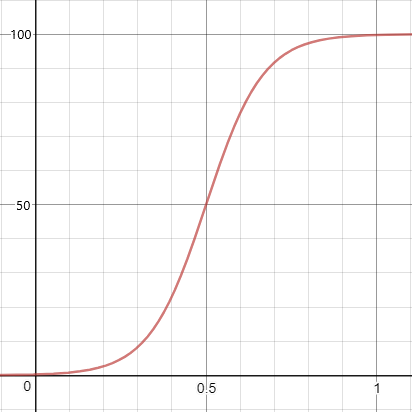
\includegraphics[width=0.8\columnwidth]{figures/Capture1}
	\caption{The force transfer function with a logistic curve}~\label{fig:figure2}
\end{figure}




\section{Implementation} 

%We designed a web-based application that was responsive to force using a JavaScript library Pressure.js \cite{pressurejs}. The library enabled force sensing across different platforms, allowing us to retain the potential to compare the techniques on different platforms. 
%
%For every task, the participants were asked locate the target object in the page using the designated technique. For tasks that required the use of traditional techniques, the ForceScroll semantics were disabled. On the other hand, the tasks that use ForceScroll techniques have access to the traditional techniques as well. This was because the gestures in ForceScroll were additional semantics to the original ones using force.
%
%During the experiment, the application used JavaScript to record how did the participant reach his target: including all the gestures he made, detection for overshoot, and the time to complete each task. The results were stored and analyzed with R.
The experiment is setup on a MacBook Pro (13-inch, 2016, resolution 2560 x 1600) with force touch enabled and run on Safari 12.0.1.

The interface is implemented with Javascript/Html/CSS with a javascript library Pressure.js\cite{pressurejs} to interact with the Force Touch events generated by Safari. The library enabled force sensing across different platforms, allowing us to retain the potential to compare the techniques on different platforms. The value of the force captured is within 0 to 1. jQuery is used to capture the trackpad events such as mouse down, mouse up, and scrolling to implement higher level function such as force scroll and force press.Other essential libraries that are used are lorem-ipsum and seedrandom. lorem-ipsum was used to generate random texts and seedrandom is used to control the randomized process.

For the test blocks, the documents and the position of target images are randomized so that participants don’t get familiar with the target location. In the recorded blocks, the document is fixed and the target images can only show up in 6 locations in the document. The images are always centered in the document and with a size of width 600px and height 400px.

The location of each chapter follows the following conditions:
\begin{itemize}
\item The length of the document: 33451px
\item The location of Chapter 1: 161px from top
\item The location of Chapter 2: 8161px from top
\item The location of Chapter 3: 17106px from top
\item The location of Chapter 4: 24707px from top
\end{itemize}

The location of targets are coded with a combination of Length and Direction. For each following distances, the target can be above or below the center of the document.

\begin{itemize}
	\item SHORT: 4000 from the center
	\item MEDIUM: 10000 from the center
	\item LONG: 15000 from the center
\end{itemize}

For tasks that required the use of traditional techniques, the ForceScroll semantics were disabled. On the other hand, the tasks that use ForceScroll techniques have access to the traditional techniques as well. This was because the gestures in ForceScroll were additional semantics to the original ones using force. This was the same for ForcePress.

During the experiment, the application used JavaScript to record how did the participant reach his target: including all the gestures he made, detection for overshoot, and the time to complete each task. The results were stored and analyzed with R. See Figure 3 for a visualization of collected data.

\begin{figure}[!h]
	\centering
	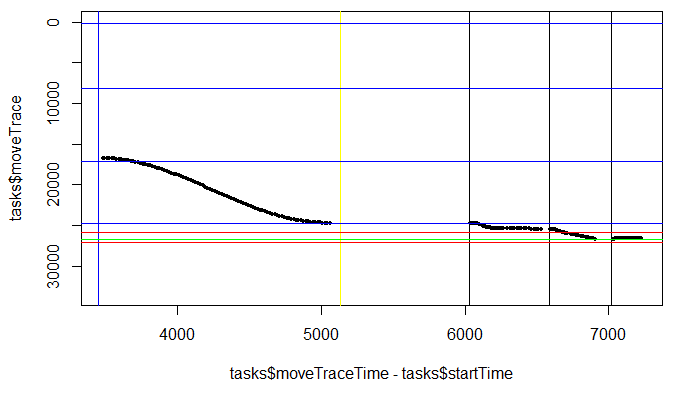
\includegraphics[width=0.9\columnwidth]{figures/Picture1}
	\caption{Visualization of one task, horizontal lines indicate locations in document, vertical lines indicate interactions of different techniques}~\label{fig:figure3}
\end{figure}

\section{Pilot}
A pilot study was performed before the experimentation to determine the speed of the auto-scroll for ForceScroll and to test the experiment procedure. Three speed levels were tested by four participants. Three participants found the speed for the auto-scroll did not affect their performance and did not prefer one speed over another. One participant chose the medium speed setting over other speed setting, but also acknowledged that the level of speed had minimum effect on his performance. We decided to keep the medium speed setting for the experiment. Another discovery was that the ForceScroll system was difficult to use, potentially due to the natural of the hardware.   


\section{Experimentation}

\subsection{Method and Apparatus}
Our experiment was conducted on a MacBook with a force-sensitive trackpad. The test software was written in JavaScript and HTML with the JavaScript library Pressure.js. The pressure applied to the trackpad was used to determine the outcome of the gesture. The default setting of the MacBook scrolling gesture was used for the traditional cases.

\subsection{Procedure, Task, and Design}
We first asked participants two 5 point likert scale questions on their familiarity with MacBook Pro trackpad and its force touch ability. We then demonstrated the operations of the each control schemes, and described how to perform each action to each participant. Once the participant understood the gestures, we let the participant practiced each technique in a test block that allowed infinite number of trials until he can perform the desired actions. We instructed the participants to perform three test blocks, one for each technique, this also let them get familiar with the experiment application interface.

Once the participants finished all practice blocks, the formal test blocks begin. At the start of each task, the interface indicated the required technique for the task. It showed the target, a picture, that the participants were required to find, and the direction of the target relative to the starting position of the display. The starting position were set to always be the center of the document. See Figure 4 for an illustration of the interface.

\begin{figure}[!h]
	\centering
	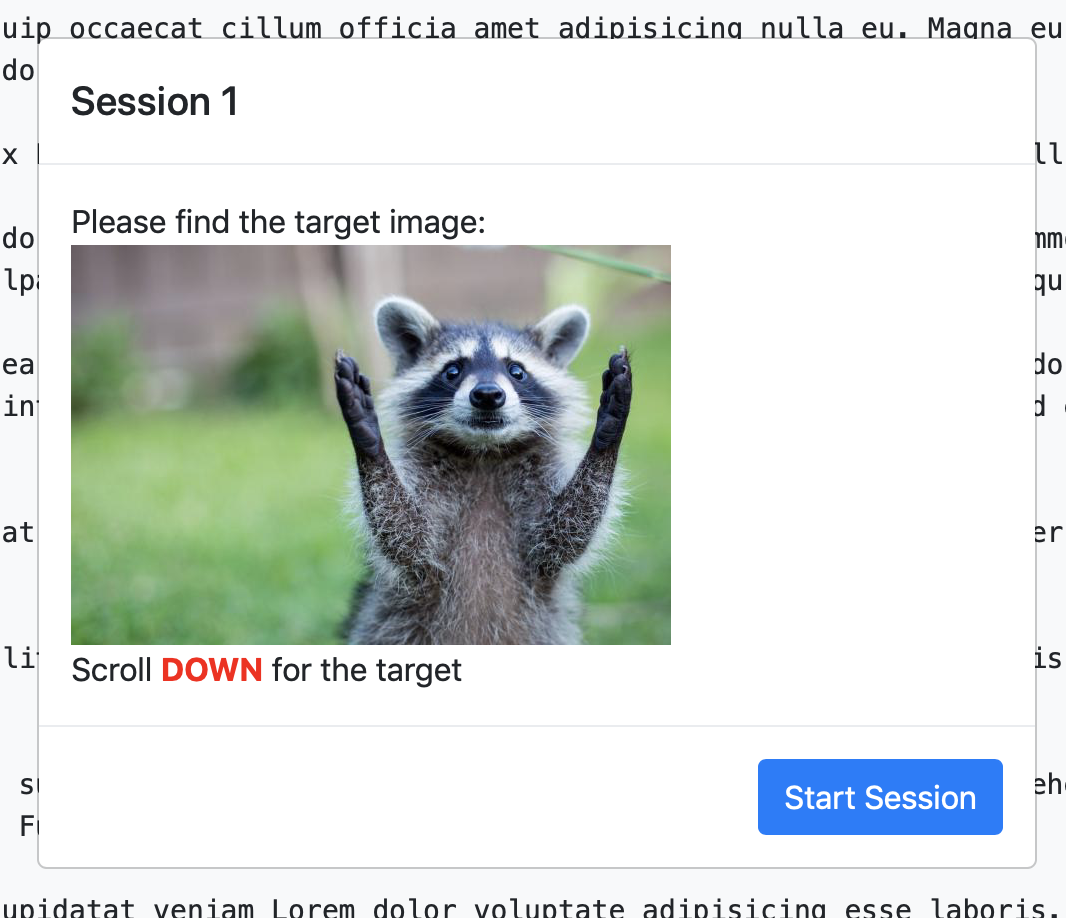
\includegraphics[width=0.7\columnwidth]{figures/figure3}
	\caption{The pop-up windows with task information}~\label{fig:figure4}
\end{figure}

Once the participants started the task, they were presented with a sidebar which indicated the current position of the display. It also indicated the target position in the document represented using a green bar, and the headers of each chapter were represented in blue bars. The sidebar was non-interactive so the participants cannot use it the traverse the document. The participants then performed the reaching task by scrolling, using the required technique, to the target location and finished the current task by clicking on the target image. Once the participants clicked on the target image, the current task was considered complete, and the participants can start a new task by clicking the ``next'' button. For a image of the application interface, see Figure 1.

The experiment used a 3x3x5 within-subjects design, the factors were: technique (Traditional, ForceScroll, or ForcePress), block (1-3, for learning effect), and distance (five out of short-up, short-down, medium-up. medium-down, long-up, and long-down). The experiment was performed following a within-group design since we expected all participants to be familiar with the traditional scrolling scheme. Testing in the traditional scheme also offered participants an opportunity to familiarize themselves with the apparatus.

The targets appeared in predetermined locations in the document, there were three different location settings: short, medium, and long. Each distance setting can appear either above the starting location or below it, thus resulting in six different target locations. Three blocks of tests were performed by each participant, in each block, the participant performed five traditional technique, five ForceScroll technique, and five ForcePress technique in order, with varying distances. For a technique in a block, the order of target location was the same for the five tasks. Different techniques in a block had different order of target locations, selected from a balanced Latin square of 6. All participants had different combinations of block orders. For example, if P1's first block order was short-up, short-down, medium-up, long-up, medium-down, its second block had the order long-down, short-up, medium-down, short-down, long-up, while the order for each block could repeat for different participants, the order between the two block never reoccur. So no other two blocks for any participant will have the order of block 1 for P1 followed by the order of block 2 for P1. The participants were given opportunity to rest between blocks.

%
%Two groups of tests were performed by each participant. The first group of tests was the traditional system test where the ForceScroll semantics was disabled. For the first ten tasks, the participants were given an on-screen arrow that indicates the position of the target object in the document relative to the displayed position of the document as each task began. The arrow was bounded to a location in the document and disappeared after being scrolled out of the screen. When each task began, a graph object was inserted into the document. The participants were asked to discover the object and click on the object to finish the task. Once a task was finished, a new task will be issued after 3 seconds. 
%
%After ten tasks, the participants were given another ten tasks, where the general position of the object was displayed on a sidebar in the window. The full length of the sidebar represented the document length, with a marker representing the currently displayed location in the document, and the sidebar could not be interacted with. The participants were again asked to discover and click on the graph object in order to finish the task. A new task was issued after 3 seconds after task completion. These 20 tasks formed the first group of the test. 
%
%The tasks in the second group, the ForceScroll tests, were identical in design and number to those in the first group, except the locations of each object were different, and the ForceScroll semantics was enabled. The participants were given one minute to rest between two groups of tests. The order of tasks within the group was different for each participant. In this group of tests, the users were instructed to use the ForceScroll system to facilitate their tasks.

Once all three blocks of tests were completed, the experiment was finished. We then asked the participants three 5 point likert scale questions on the ease of use for each of the three techniques. The participants were not compensated.

The independent variables in the experiment were \textit{Traditional, ForceScroll, or ForcePress}, \textit{Distance to Target}, and \textit{Block}. The \textit{Distance to Target} was calculated by the number of pixels. Dependent variables investigated were \textit{Time}, \textit{Total number of interaction}, \textit{Overshoot distance}, \textit{Overshoot number}, and \textit{Longest overshoot}. The \textit{Overshoot Distance} was calculated by the number of pixels between the bottom (or top) of the screen and the top (or bottom) of the object. The overshoot occurred when the participants scrolled the target object out of the display window, the distance of the overshoot is calculated once the participant stop the scrolling and started to backtrack.   

\subsection{Participants}
12 university graduate students participated in the experiment. According to the 5-point likert scale questions, while 7 out of the 12 participants were familiar with MacBook trackpad (mean = 3.42), no participants had extensive experience with MacBook trackpad's force-sensing ability (mean = 1.25). Only two of them claimed to have any experience with MacBook trackpad's force-sensing ability (P2 who answered 3 and P3 who answered 2).
    
\subsection{Research Hypotheses}

We proposed eight research hypotheses for the ForceScroll system:

\begin{itemize}
	\item \textbf{H1}: The ForceScroll system requires less time to complete a reaching task compared with traditional system.
	\item \textbf{H2}: The ForceScroll system requires less interaction to complete a reaching task compared with traditional system.
	\item \textbf{H3}: The ForceScroll system produces less overshoot compared with traditional system.
	\item \textbf{H4}: The ForceScroll system is more comfortable to use compared with traditional system.
\end{itemize}

Our dependent variable was the time required to finish each task, the total distance of overshoot.

We proposed three research hypothesis (\textbf{H5}, \textbf{H6}, \textbf{H7}, \textbf{H8}) for the ForcePress system, they were identical to the hypothesis for the ForceScroll system.

According to our pilot study, we proposed 4 additional research hypotheses, which stated:
\begin{itemize}
	\item \textbf{H9}: The ForcePress system requires less time to complete a reaching task compared with the ForceScroll system.
	\item \textbf{H10}: The ForcePress system requires less interaction to complete a reaching task compared with the ForceScroll system.
	\item \textbf{H11}: The ForcePress system results in less overshoot compared with the ForceScroll system.
	\item \textbf{H12}: The ForcePress system is more comfortable to use than the ForceScroll system.
\end{itemize}

\subsection{Results}
\subsubsection{Time}
\textit{Time} is the dependent variable used to determine H1, H5, and H9. It indicates the time spent on performing one reaching task. It is the time between the participant clicking on ``start session'' and clicking on the target image. Figure 5 shows the mean time for each technique and distance.
\begin{figure}[!h]
	\centering
	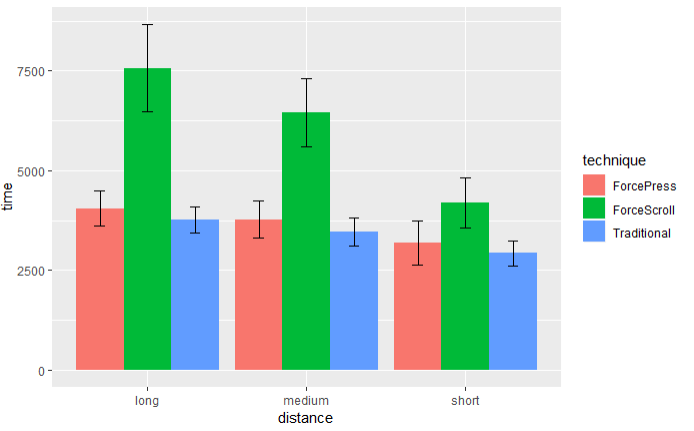
\includegraphics[width=0.8\columnwidth]{figures/figure4}
	\caption{Mean time for each technique and distance, after block 1 removal}~\label{fig:figure5}
\end{figure}
 
A Repeated measures ANOVA revealed a significant effect of block on \textit{time} (F(1.15, 12.66) = 10.19, p = 0.006). Since the data is nonparametric, an aligned rank transform was performed to transform the data, a subsequent ANOVA confirmed this discovery (p < 0.001). A wilcox post-hoc analysis revealed a significant reduction in \textit{time} between block 1 and the two subsequent blocks (p < 0.0005, block 1: 5.2, 2: 4.5, 3: 4.2). As a result, we removed block 1 for \textit{time} analysis. ANOVA revealed significant effects of technique (F(2,22)=39.28, p < 0.001) and distance (F(2,22)=22.40, p < 0.001) on \textit{time}. Aligned rank transformed data confirmed these findings (F(2,187)=129.82, p < 0.0001 and F(2,187)=56.89, p < 0.0001). It also indicated a significant interaction between technique and distance (p < 0.005). A subsequent wilcox post-hoc analysis showed a significant increase in \textit{time} for ForceScroll compared with the other techniques (p < 0.0005) as distances became longer. \textit{time} for each technique also significantly increased between short distance and long distance (p < 0.0005), while the increase and decrease from medium distance to both short and long distance were not significant. A Friedman test was performed since the data was nonparametric to confirm the result ($x^{2}$(8) = 62.9, p < 0.0001).

As a result of the above analysis, H1 and H5 were rejected. The two new technique did not reduce the time required for participants to reach the target. In case of ForceScroll, it required significantly more time to reach the target. In case of ForcePress, the difference was insignificant, but ForcePress required more time than traditional technique. This result confirmed H9, ForcePress is faster compared with ForceScroll.


\subsubsection{Number of interaction}
\textit{Number of interaction} is the dependent variable used to determine H2, H6, and H10. It represents the total amount of actions the participant performed to finish the task. The interactions included the interaction technique being tested and all traditional interactions. Figure 6 shows the mean number of interaction for each technique and distance. 
\begin{figure}[!h]
	\centering
	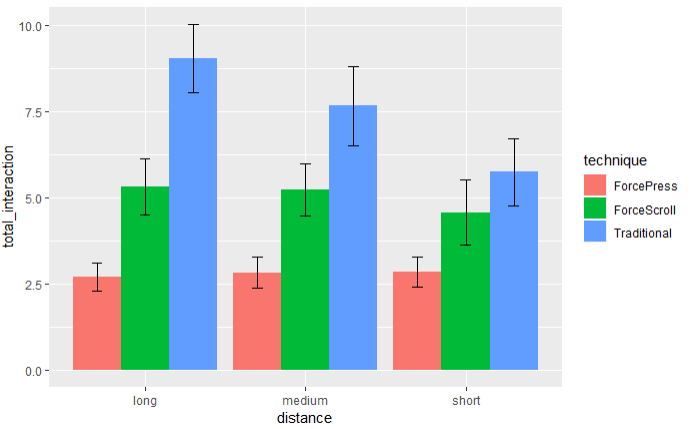
\includegraphics[width=0.8\columnwidth]{figures/figure5}
	\caption{Mean number of interaction for each technique and distance, after outliers were removed}~\label{fig:figure6}
\end{figure}

ANOVA prior and after aligned rank transform showed no significant effect of block on \textit{interaction}, ANOVA prior to transform showed a significant effect of technique (F(2,22)=26.86,p<0.001) and distance (F(2,22)=16.37,p<0.001) on \textit{number of interaction}, and a significant interaction between technique and distance (F(4,44)=8.02,p<0.001). ANOVA on transformed data confirmed this finding (p<0.001 for all). A wilcox rank test was performed for post-hoc analysis, traditional technique resulted in significantly more interactions compared with the other techniques (p<0.0001, Traditional:9.8, ForceScroll:5.5, ForcePress:2.8), and ForceScroll had significantly more interactions compared with ForcePress at long and medium distances (p<0.001, long: ForcePress:2.6, ForceScroll:6.3, medium: ForcePress:2.8, ForceScroll:5.3). The distance had no significant effect for all technique except for traditional technique, whose interactions at short distance was significantly less compared with at long distance (p<0.001, short:6.6, long:12.3). A Friedman test was performed since the data was nonparametric to confirm the result ($x^{2}$(8) = 60.941, p < 0.0001).% While post-hoc wilcox rank test did not find significant different between ForcePress and ForceScroll at medium and short distance, the pattern was the same.

As a result of the above analysis, H2 and H6 were confirmed. The two new techniques reduced the amount of interactions needed to reach the target (p < 0.0005 for long and medium distance, not significant for short distance but with smaller mean values), especially for ForcePress or for longer distance tasks. The data also partially confirmed H10, as ForcePress required less interaction compared with ForceScroll in long and medium (p < 0.0001), but the reduction was insignificant for short distance (p = 0.17).

\subsubsection{Overshoot distance}  
\textit{Overshoot distance} is the dependent variable used to determine the error for each technique for H3, H7 and H11. It is the total distance for all overshoots. See Figure 7 for the mean overshoot distance for each technique and distance.

\begin{figure}[!h]
	\centering
	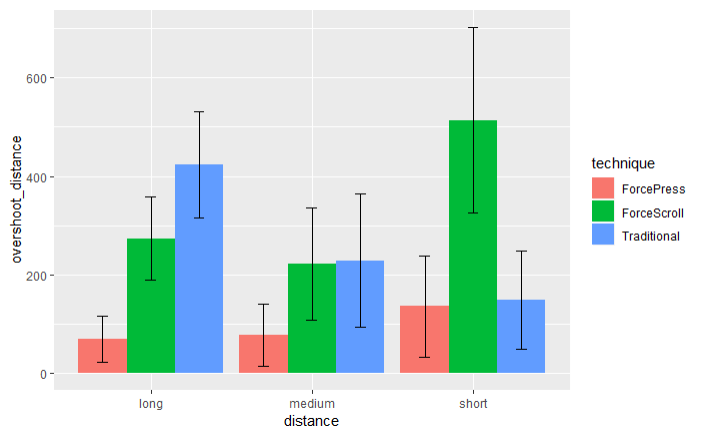
\includegraphics[width=0.8\columnwidth]{figures/figure6}
	\caption{Mean number of total overshoot distance for each technique and distance, after outliers were removed, note the large confident interval}~\label{fig:figure7}
\end{figure}

Once more, ANOVA prior and after aligned rank transform showed no significant effect of block on \textit{overshoot distance}. ANOVA prior to aligned rank transform showed a significant effect of technique (F(1.27,13.93)=9.72,p<0.01) on \textit{overshoot distance}, and a significant interaction between technique and distance (F(4,44)=5.01,p<0.005). ANOVA on transformed data confirmed this finding (p<0.005 for all), and indicated a significant effect of distance (p<0.001) on \textit{overshoot distance} and a significant interaction between distance and block (p<0.005). A wilcox rank test was performed for post-hoc analysis. There was no evidences of the interaction between distance and block, and no evidences of significant effect from distance. The overshoot distance for long distance traditional technique was significantly larger compared with long distance ForcePress (p<0.005, Traditional: 438.36, ForcePress: 78.02). Short distance ForceScroll resulted in a significantly longer overshoot distance compared with both traditional and ForcePress techniques(p<0.005, Traditional:147.54, ForceScroll:986.83, ForcePress:140.76). Overall, the \textit{overshoot distance} for ForcePress is much smaller compared with other techniques(p<0.0001, Traditional:323.37, ForceScroll:582.03, ForcePress:98.6). A Friedman test was performed since the data was nonparametric to confirm the result ($x^{2}$(8) = 26.359, p < 0.001).

As a result, H7 was confirmed. H3 was confirmed for long and medium distance tasks, but not true for short distance tasks. H11 was also confirmed (p < 0.0001).  

\subsubsection{Overshoot number and Longest overshoot}
\textit{Overshoot number} is the amount of overshoot and \textit{Longest overshoot} is the distance of the longest overshoot for all overshoots during one task. The same analysis process was followed by both dependent variables. The effects found for both variables were similar to the findings revealed during the analysis for the total overshoot distance. After reviewing the findings, we believed that the total overshoot distance was sufficient to validate H3, H7, and H11.    

\subsubsection{Ease of use}
The three 5-point likert scale questions asked after the experiment were used to determine whether the technique was easy to use. The mean value for each question among twelve answers was used. See Table 1 for the results.

\begin{table}[h]
	\begin{tabular}{|l|l|l|}
		\hline
		Traditional & ForceScroll & ForcePress \\ \hline
		4.42        & 2.42        & 4.42       \\ \hline
	\end{tabular}
\end{table}

For the twelve participants, the ForcePress technique was as easy to use as the traditional technique, while the ForcePress technique was difficult to use. This means H4 is false, H8 is true, and H12 is true.

\subsection{Discussion}
Our experiments showed that both new techniques failed to improve the scrolling speed. For ForceScroll, the difficulty in the technique's activation could be an important factor, as participants spend times to activate the auto-scroll. During the experiment, we noticed most participants used traditional technique only after an overshoot had occurred. During the design of the technique, we imagined the users would use the ForceScroll technique to cover distances by quickly moving through chapters, and navigate to the target location using traditional technique. Enforce this scheme could affect the overall time, and is worth further investigation. The difficulty in activating the auto-scroll and the uncomfortable control also need to be addressed, access to the MacBook trackpad's lower level controls may be needed. On a positive note, the ForceScroll technique successful reduced the number of interactions needed, especially for longer distances. This is especially useful for users who have limited mobility on their fingers.

For ForcePress, although it is not significantly faster, and in most cases slower, when compared with the traditional technique, it is also not much slower. This could be the effect of the force transfer function, a dedicated study for fine-tuning the transfer function should benefit the technique greatly. The ForcePress is great in reducing the number of interaction needed. In fact, for all distances, the number of interaction required in the ForcePress scheme is very close. This is due to the continuous nature of the techniques, participants can reach their target using one ForcePress most of the time. We are somewhat surprised to learn that for our participants the ForcePress is as comfortable as the traditional technique, one participant even rate ForcePress to be more comfortable than the traditional technique. This sharp distinction between ForceScroll and ForcePress is likely influenced by the present of the Force Click, as it is required to activate the ForceScroll, but has no special meaning for ForcePress.  

For overshoot distances, the large amount of overshoot for traditional technique at long distance could be the result of mouse acceleration, and the large amount of overshoot for short distance overshoot can potentially be counteracted by enforcing the previously mentioned control scheme.

There are some limitations to our technique and study. We achieved all functionalities with a JavaScript library instead of accessing Apple's API for the trackpad. There are likely some overhead in our current approach. For the study, we need more data. Our limited data prevented us from removing outliers in some cases, as doing so resulted in missing cells during ANOVA. We also need to expend the participants to include more demographic, and test other devices other than the one MacBook used in our current study.  
\section{Future Work}
For future works, we would like to iterate on the ForceScroll and ForcePress techniques. For ForceScroll, we would try to implement the technique using Apple's API for the trackpad, instead of using a JavaScript library. For ForcePress, an interesting idea, proposed by Dr. Casiez, is to implement the pressing at the end of a traditional scroll or swipe action, and the direction of the action will decide the direction of ForcePress. A new user study will involves a larger demographic of participants, and each participants will be asked to complete more tasks. We would also like to study the effect of the direction of target on task completion time and accuracy.  

    
\section{Conclusion}
In this paper, we proposed two novel interaction techniques that can be used to improve the reading speed by increasing the users' scrolling speed, allowing them to reach desired location faster. We performed a user study to test the efficiency and accuracy of the two techniques. The ForceScroll technique did not perform well, as it takes longer than traditional technique to reach a target, it had limited success in reducing the number of interaction for longer distances, and did not reduce the overshoot distance when compared with traditional technique. It is also uncomfortable to use. ForcePress, on the other hand, was more successful than ForceScroll, although it did not increase the speed, it was also not significantly slower. It succeed in reducing the number of interactions, and generally resulted in smaller overshoot distance. It is also as comfortable to use as the traditional technique.      

% BALANCE COLUMNS
\balance{}

% REFERENCES FORMAT
% References must be the same font size as other body text.
\bibliographystyle{SIGCHI-Reference-Format}
\bibliography{sample}

\section{Appendix}
The task was divided between the two authors. For the implementation. Sung-Shine Lee took the main responsibility due to his expertise with JavaScript and access to a compatible device. For the experimentation, both authors conducted the study together. Ruoteng Ma analyzed the data and Sung-Shine validated the results. Ruoteng Ma took the main responsibility of writing the paper, both the final paper and each milestones, Lee also contributed to the writing by editing and proof-reading. The experiment structure and procedure were designed by both authors together, with the structure and balancing initially designed by Ruoteng Ma, later checked and edited by Sung-Shine. The video was made by Ruoteng Ma.  

\end{document}

%%% Local Variables:
%%% mode: latex
%%% TeX-master: t
%%% End:
